\documentclass[simplex.tex]{subfiles}
% NO NEED TO INPUT PREAMBLES HERE
% packages are inherited; you can compile this on its own

\onlyinsubfile{
\title{NeuroData SIMPLEX Report: Reduced Dimension Clustering}
}

\begin{document}
\onlyinsubfile{
\maketitle
\thispagestyle{empty}

The following report documents the progress made by the labs of Randal~Burns and Joshua~T.~Vogelstein at Johns Hopkins University towards goals set by the DARPA SIMPLEX grant.

%%%% Table of Contents
\tableofcontents

%%%% Publications
\bibliographystyle{IEEEtran}
\begin{spacing}{0.5}
\section*{Publications, Presentations, and Talks}
%\vspace{-20pt}
\nocite{*}
{\footnotesize	\bibliography{simplex}}
\end{spacing}
%%%% End Publications
}

\subsection{Batch effect removal in dimension reduction of multiway array data}

Batch effects are unwanted random variations caused by different data sources and experimental conditions. Generalized linear random effects model is effective to mitigate these confounders in traditional low dimensional data; however, there is a lack of such tool for high dimensional and multiway array data. While tensor factorization is routinely used for dimension reduction, due to the sharing of factors among all batches, the batch effects quickly populate the low dimensional core and confound the signal. In this research, we propose a different strategy by letting factor matrices vary over batches, while leaving the remaining variation in the core. This allows capturing sophisticated batch effects, while retaining the low rank structure for describing signal. To allow estimation with flexible factors, we utilize a hierarchical random effects model to borrow information among the batches. An efficient closed-form expectation conditional maxmization strategy is developed for rapid estimation. We focus the application on the joint diagonalization of brain connectivity data obtained from different sources. Our model show substantial gains in the simulations and application over the alternatives.



\begin{figure}[h!]
\begin{cframed}
\centering
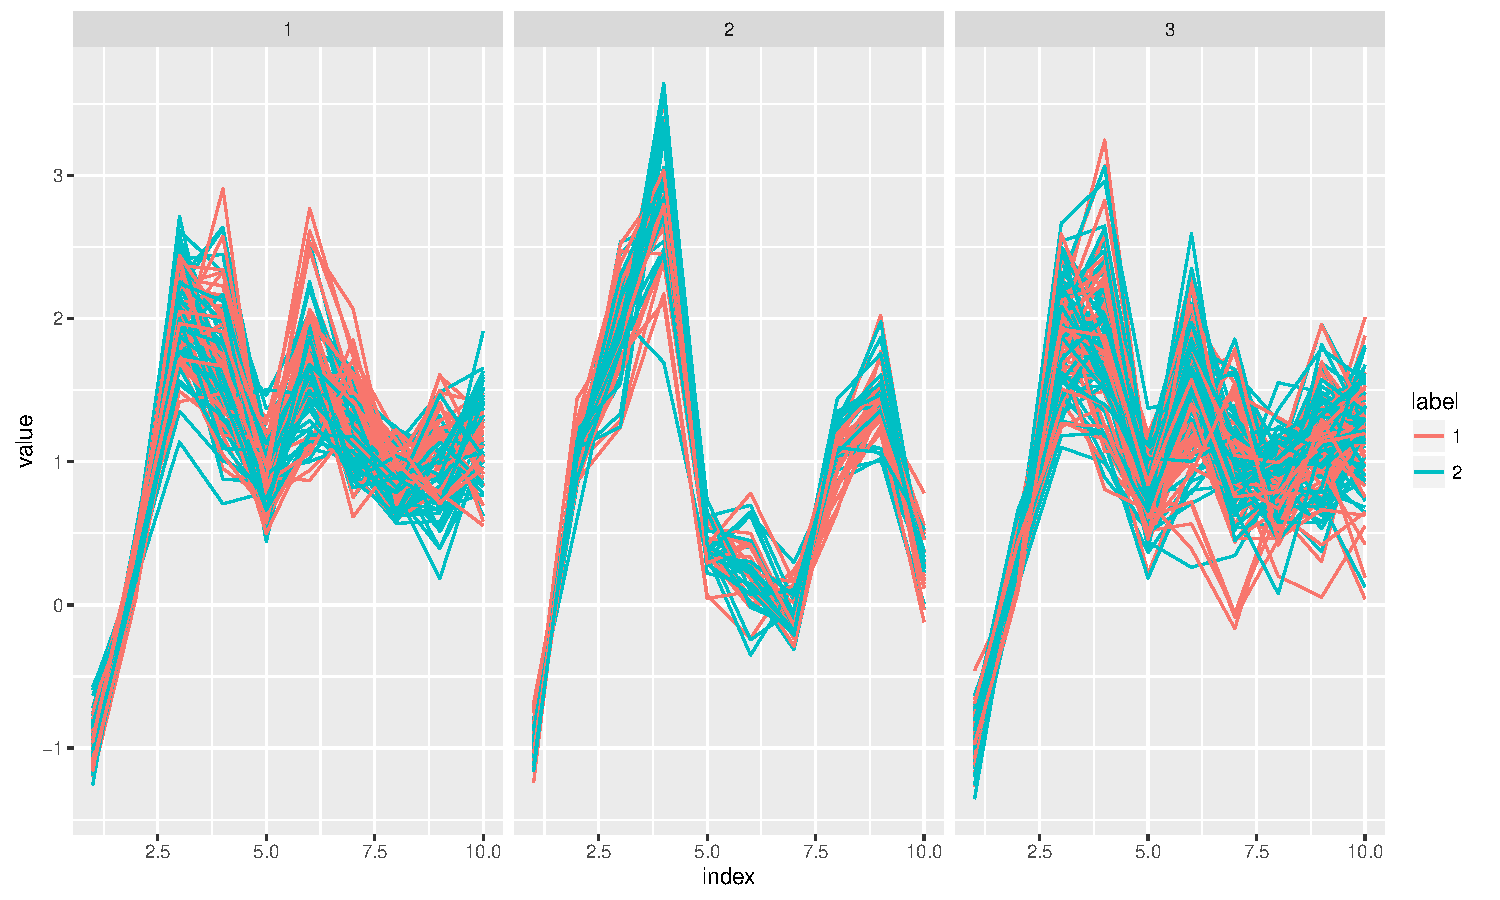
\includegraphics[width=0.45\textwidth]{../../figs/BE_not_removed_data}
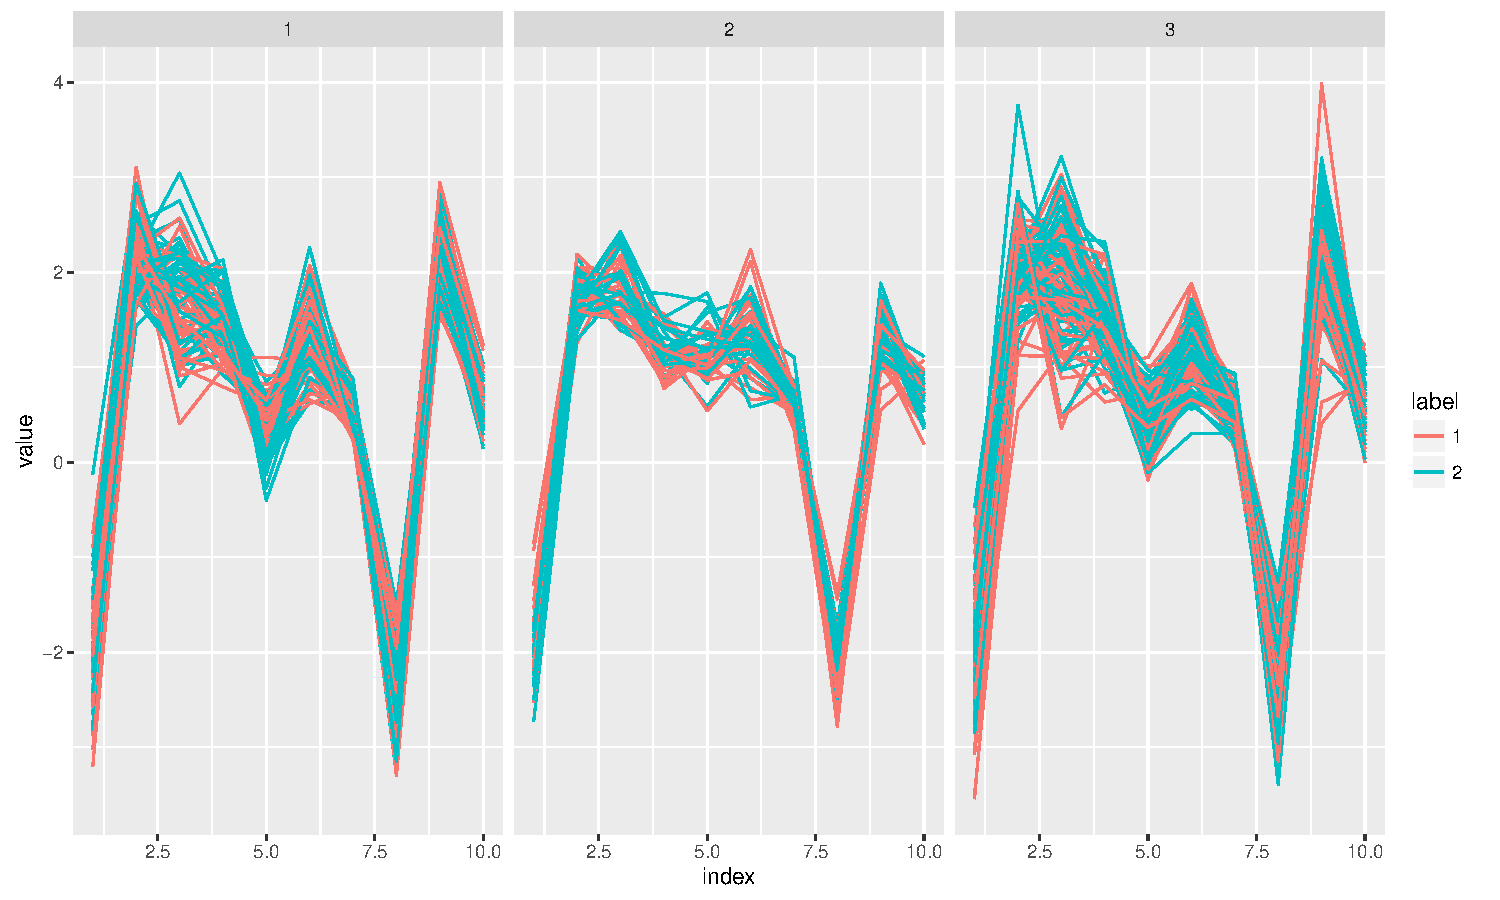
\includegraphics[width=0.45\textwidth]{../../figs/batch_removal_data}
\caption{The batch effect removing model reduce the group random variation of the second group, and makes it more similar to the others.}
\label{fig:arc}
\end{cframed}
\end{figure}


\end{document}
